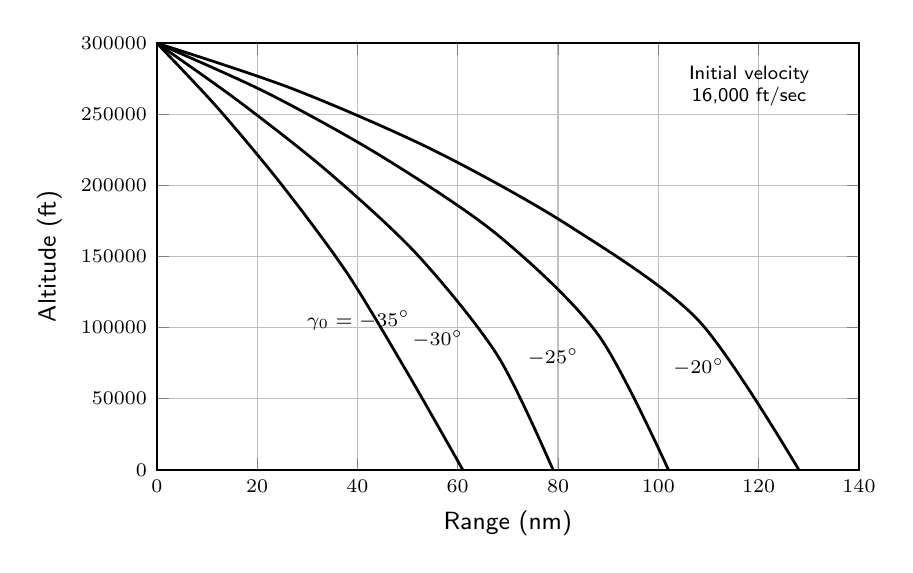
\begin{tikzpicture}
\begin{axis}[
  width=10.5cm,height=7.0cm,
  xmin=0,xmax=140,ymin=0,ymax=300000,
  xtick={0,20,40,60,80,100,120,140},
  ytick={0,50000,100000,150000,200000,250000,300000},
  grid=major,
  axis line style={line width=0.8pt},
  tick label style={font=\scriptsize},
  label style={font=\sffamily\small},
  xlabel={Range (nm)},ylabel={Altitude (ft)},
  scaled y ticks=false,
  yticklabel style={/pgf/number format/fixed,/pgf/number format/1000 sep={}},
]
  \addplot[line width=1.0pt,smooth] coordinates {(0,300000) (12,255000) (25,200000) (38,138000) (50,68000) (61,0)};
  \addplot[line width=1.0pt,smooth] coordinates {(0,300000) (16,260000) (34,210000) (52,151000) (68,80000) (79,0)};
  \addplot[line width=1.0pt,smooth] coordinates {(0,300000) (22,265000) (45,220000) (68,165000) (88,95000) (102,0)};
  \addplot[line width=1.0pt,smooth] coordinates {(0,300000) (27,268000) (55,225000) (82,172000) (108,105000) (128,0)};
  \node[font=\sffamily\scriptsize,anchor=west] at (axis cs:28,105000) {$\gamma_0=-35^\circ$};
  \node[font=\sffamily\scriptsize,anchor=west] at (axis cs:49,92000) {$-30^\circ$};
  \node[font=\sffamily\scriptsize,anchor=west] at (axis cs:72,79000) {$-25^\circ$};
  \node[font=\sffamily\scriptsize,anchor=west] at (axis cs:101,72000) {$-20^\circ$};
  \node[font=\sffamily\scriptsize,align=center,anchor=east] at (axis cs:132,270000) {Initial velocity\\16,000 ft/sec};
\end{axis}
\end{tikzpicture}
